\documentclass[tikz,border=8pt]{standalone}
\usetikzlibrary{shapes.gates.logic.US,positioning}
\begin{document}
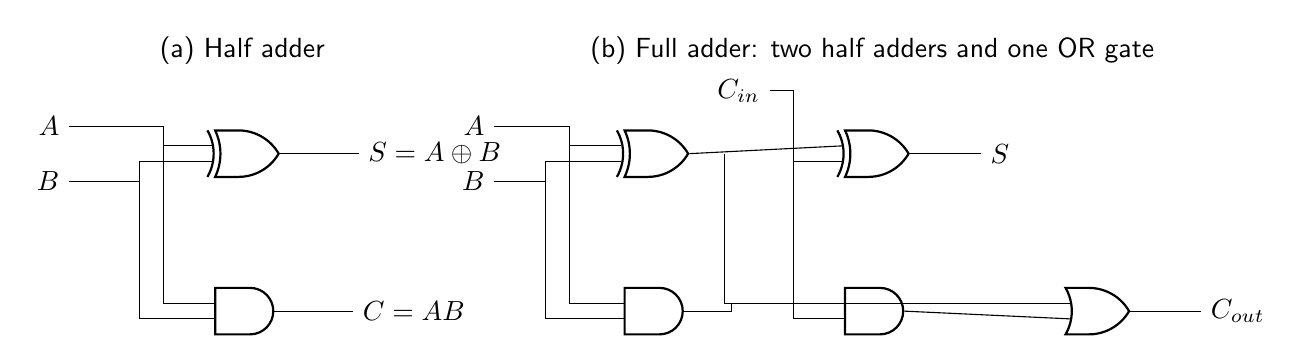
\begin{tikzpicture}[every node/.style={font=\sffamily}, gate/.style={draw,thick,logic gate inputs=nn}]
  \node[xor gate US,gate] (hx) at (2.0,3.0) {};
  \node[and gate US,gate] (ha) at (2.0,1.0) {};
  \coordinate (haA) at (-.2,3.35);
  \coordinate (haB) at (-.2,2.65);
  \draw (haA) node[left]{$A$} -- (1.0,3.35) |- (hx.input 1);
  \draw (1.0,3.35) |- (ha.input 1);
  \draw (haB) node[left]{$B$} -- (.7,2.65) |- (hx.input 2);
  \draw (.7,2.65) |- (ha.input 2);
  \draw (hx.output) -- ++(1.0,0) node[right]{$S=A\oplus B$};
  \draw (ha.output) -- ++(1.0,0) node[right]{$C=AB$};
  \node[above=7mm of hx] {(a) Half adder};

  \node[xor gate US,gate] (x1) at (7.2,3.0) {};
  \node[xor gate US,gate] (x2) at (10.0,3.0) {};
  \node[and gate US,gate] (a1) at (7.2,1.0) {};
  \node[and gate US,gate] (a2) at (10.0,1.0) {};
  \node[or gate US,gate] (o1) at (12.8,1.0) {};
  \draw (5.2,3.35) node[left]{$A$} -- (6.15,3.35) |- (x1.input 1);
  \draw (6.15,3.35) |- (a1.input 1);
  \draw (5.2,2.65) node[left]{$B$} -- (5.85,2.65) |- (x1.input 2);
  \draw (5.85,2.65) |- (a1.input 2);
  \draw (x1.output) -- (x2.input 1);
  \draw (x1.output) ++(.45,0) |- (a2.input 1);
  \draw (8.7,3.8) node[left]{$C_{in}$} -- (9.0,3.8) |- (x2.input 2);
  \draw (9.0,3.8) |- (a2.input 2);
  \draw (x2.output) -- ++(.9,0) node[right]{$S$};
  \draw (a1.output) -- ++(.6,0) |- (o1.input 1);
  \draw (a2.output) -- (o1.input 2);
  \draw (o1.output) -- ++(.9,0) node[right]{$C_{out}$};
  \node[above=7mm of x2] {(b) Full adder: two half adders and one OR gate};
\end{tikzpicture}
\end{document}
